\documentclass[12pt]{article}

\usepackage{tabularx} 
\usepackage{subcaption}
\usepackage{pdfpages}
\usepackage{amsbsy}
\usepackage{amssymb}

\usepackage{graphicx}
\graphicspath{{Pictures/}}
\usepackage[longnamesfirst]{natbib}
\usepackage{amsmath}
\usepackage{enumerate}

\usepackage{relsize}
\usepackage{color}
\usepackage{listings}

\usepackage{times}
\usepackage{amsmath}
\usepackage{amssymb}
\usepackage[margin = 2.5cm]{geometry}

\renewcommand{\thesection}{\Roman{section}}
\renewcommand{\thesubsection}{\Alph{subsection}}
\renewcommand{\thesubsubsection}{\arabic{subsubsection}}
\newcommand*{\R}{\textsf{R}$~$}

\let\svthefootnote\thefootnote

\begin{document}
\begin{center}
	\Large Seen to Be Done \\ {\large Visually exploring racial bias in jury selection}
	\\ \vspace{0.5cm}
	\large Chris Salahub\let\thefootnote\relax\footnotetext{csalahub@uwaterloo.ca; University of Waterloo, 200 University Ave. Waterloo, Canada. The author thanks Prof. Dr. Marloes Maathuis at ETH Z\"urich for her advice and guidance.}
	\let\thefootnote\svthefootnote
\end{center}
 
\pagenumbering{arabic}%--- switch back to standard numbering

In early 2018, a landmark court case changed Canadian legal practice permanently. Days after the verdict of \emph{R. v. Stanley}, legislation was introduced to remove a process in Canadian jury trials which predates the country itself. It was only a few months later that the offending practice, the peremptory challenge, was abolished in Canada.

Racial optics were at the core of this controversy. Gerald Stanley, a white man, was acquitted of the second degree murder of Colten Boushie, a First Nations man, by an all-white jury. Moreover, peremptory challenges were used by Stanley's legal team on five separate occasions to remove First Nations individuals from the jury. Many community members found this exclusion unconscionable and so brought the trial to the attention of the national media, which prompted the legislative response of the Liberal government.

This monumental change was not without precedent, however. Peremptory challenges were abolished in the United Kingdom in 1988 following the controversial Cyprus spy trial, and have been curtailed in the United States since \emph{Batson v. Kentucky} in 1986. \emph{R. v. Stanley} is now in the dubious company of these other controversies. The same theme repeats throughout: ``bias.'' Before we can explore this bias, however, we need to understand peremptory challenges and jury trials at a basic level.

\subsection*{Jury trials and peremptory challenges}

It would take a much longer article to capture the full breadth of jury selection methods. They change readily by both jurisdiction and crime. Generally, however, the steps are as follows.

\begin{enumerate}
  \item Eligible individuals are selected at random from the population using a list of eligible jurors. The sampled individuals are called the \textit{venire}.
  \item The venire is presented to the court, either all at once or sequentially.
  \item The prosecution, arguing against the accused, and defence, arguing on behalf of the accused, question the presented venire members. There are three possible outcomes:
    \begin{enumerate}
      \item The venire member is \textit{struck} with cause, i.e. chosen \emph{not} to serve on the jury for a reason provided by either the prosecution or defence and admitted by the judge.
      \item The venire member is struck by \textit{peremptory challenge} by either the prosecution or defence. Peremptory challenges do not require a reason, and so each side has a limited number.
      \item The venire member is accepted onto the jury.
    \end{enumerate}
  \item Steps (a)-(c) are repeated until the desired jury size is reached, typically 12.
\end{enumerate}

It is surprising that a process which values arguments based on evidence as highly as the legal system gives any opportunity for privileged strikes at all. It is less surprising that these peremptory challenges cause regular controversy wherever they are exercised.

In the United States, the case of \emph{Batson v. Kentucky} and \emph{Swain v. Alabama} carry the most weight. In this case, not a single black juror had sat on a jury in Kentucky in the previous 15 years, despite composing 26\% of the jury-eligible population. In Swain's trial, six of the eight black venire members were rejected by prosecution peremptory challenges, and the other two removed for cause, leaving not a single black juror to judge Swain, a black man.

Racial controversies have also been present in Canada before \textit{R. v. Stanley}. Abolition of the peremptory challenge due to alleged racial bias against First Nations venire members was recommended by the Manitoba Aboriginal Justice Implementation Commission of 1999. This sentiment was echoed in the 2013 Iacobucci Report on First Nations representation in Ontario juries.

Despite these recommendations and the legal changes in the United States, peremptory challenges are defended as a key component of the jury selection process by some. The modern defence is exemplified by Justice Byron R. White's opinion in \emph{Swain v. Alabama}:

\begin{quote}
The function of the challenge is ... to eliminate extremes of partiality ... [and] assure the parties that the jurors ... will decide on the basis of the evidence ... In this way, the peremptory satisfies the rule that ... ``justice must satisfy the appearance of justice.''
\end{quote}

This justification calls back the famous words of Lord Chief Justice Hewart in \textit{R. v. Sussex Justices}: ``justice should not only be done, but should manifestly and undoubtedly be seen to be done''.

Without data, seeing whether justice is done over time is impossible. Here, we are presented with a difficulty. We cannot know the reason for any individual peremptory challenge, its privileged nature obscures it. Instead, we can only analyse the data that has been collected. The author is heavily indebted to \citeauthor{JurySunshineProj}; \citeauthor{StubbornLegacy}; and \citeauthor{PerempChalMurder}. These authors shared their data freely with the author, providing him with a wealth of data to analyse.

\subsection*{The data}

Of course, analysing this data starts by inspecting its collection. 
\cite{JurySunshineProj} has the most extensive data set of the three. It contains jury data for almost all felony trial cases in North Carolina in the year 2011, providing simple demographic characteristics and trial information for 29,624 individuals summoned for jury duty in 1,306 trials. The relevant case data recorded were the presiding judge, prosecutor, defence lawyer, defendant, venire members, charges, verdict, and sentence. For venire members, the collected data included the outcome -- struck with cause, struck by peremptory challenge, or retained on the jury -- of the venire member. Using public voter databases, bar admission records, and judge appointment records, the data also included race, gender, and political affiliation data for the venire members, lawyers, defendants, and judges.

\cite{StubbornLegacy} cover fewer cases with more limited scope. This study, also based in North Carolina, detailed the trials of inmates on death row as of July 1, 2010, yielding a total of 173 cases. As in the Jury Sunshine study, variables recorded for each case are the peremptory challenges, venire members, presiding judge, prosecutor, and defence lawyer. Unlike the Jury Sunshine study, detailed verdict and charge information was not collected, as the pre-selection criteria of death row inmates made the verdict clear, and the death penalty only applies to a limited number of serious crimes.

A critical difference between the Stubborn data and the Jury Sunshine data is the exclusion of venire members removed with cause in the Stubborn data. This was motivated by the analysis of the study, which focused on the differences between defence and prosecution peremptory challenges. Less critically, the Stubborn data set lacks data on political affiliation, which serves as a barrier to the comparison of this data to the Sunshine data on an identical basis.

\cite{PerempChalMurder} collected a similar data set to \cite{StubbornLegacy} using similar means. Court files such as the juror questionnaire, voter registration, and census data were all used to complete juror demographic information for 317 venires consisting of 14,532 venire members in Philadelphia capital murder cases between 1981 and 1997. It should be noted that this data included only those jurors kept or peremptorily struck, venire members struck for cause were not included. This data had a number of departures from the Sunshine and Stubborn data. It lacked racial information as detailed as either and recorded no information about political affiliation, further limiting the potential for direct comparison between all three data sets.

The \R code used to perform the analysis and generate all figures is publicly available on GitHub at github.com/Salahub/peremptory\_challenges.

\subsection{Visualisation}

First, consider the simple unconditional probabilities of removal by peremptory challenge by race in all data sets, shown in Table \ref{tab:margrace}. These probabilities are different, but not greatly so. Indeed, the trend of higher probabilities for the removal of white jurors across all data sets is perhaps counter-intuitive given the history of controversy in the United States. In any case, the small magnitude of these differences suggests only a weak racial bias at the aggregate level.

\begin{table}[h!]
  \centering
  \caption[Strike Rate by Race]{\footnotesize The conditional probability of a venire member being struck peremptorily by venire member race across data sets. Note that the Philadelphia trial data only indicated black and non-black venire members and so only two numbers can be reported.} \label{tab:margrace}
  \begin{tabular}{|c|c c c|} \hline
    \textit{Data} & \textit{Black} & \textit{Other} & \textit{White} \\ \hline
    Sunshine & 0.23 & 0.24 & 0.25 \\
    Sunshine Capital & 0.22 & 0.27 & 0.27 \\
    Stubborn & 0.65 & 0.36 & 0.66 \\ 
    Philadelphia & 0.67 & \multicolumn{2}{c|}{0.68} \\ \hline
  \end{tabular}
\end{table}

This table also demonstrates some of the drawbacks of tables. While excellent at communicating specific values, tables do not provide a sense of trends or patterns without careful engagement by the reader. This barrier limits comparisons and the impact of our data. Instead, we might want to develop a custom visualisation to compare these data sets.

Based on the history of peremptory challenge controversy, we want to visualise the joint and marginal distributions of three variables: venire member race, defendant race, and outcome (whether a venire member was struck and how). We can view this as a visualisation to test a specific hypothesis:

\begin{equation}
  \label{eq:vishyp}
  O | O \neq \text{Kept}, R, E \sim Unif(\{\text{Prosecution
    Struck, Defence Struck, Struck with Cause}\})
\end{equation}

Where $O, R, E$ are random variables representing the disposition, venire member race, and defendant race, respectively. In words: the conditional distribution of strikes given a case's racial combination is uniform. This implies that strikes with cause, defence peremptories, and prosecution peremptories all occur with the same probability for each racial combination. In other words, the hypothesis is that all parties in the court pursue an identical strike strategy across all venire member and defendant race combinations, one that is consistent with their justified strikes. This specific hypothesis motivates the ``mobile plot'' of Figure \ref{fig:racedefmob} to compare the strike dispositions of venire members by their race and the defendant race for the Sunshine data. So named because it has a slight resemblence to the mobiles hung above a babies' cribs.

\begin{figure}[!h]
  \centering
  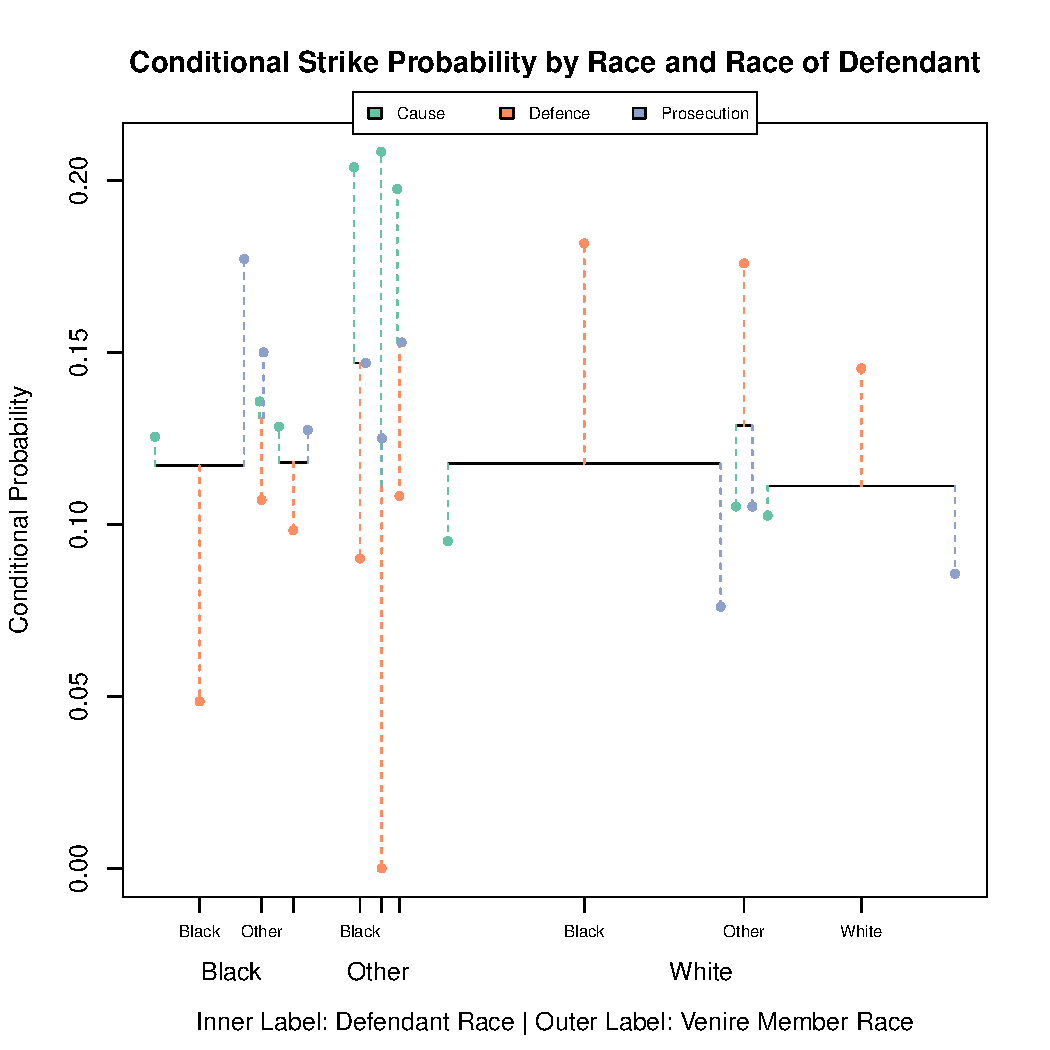
\includegraphics[width=0.7\textwidth]{RaceParCoord}
  \caption[A mobile plot of Sunshine strikes by racial combination]{\footnotesize The conditional probability of strike disposition given the
    venire member and defendant race for the Sunshine data set. Expected values are represented by the horizontal black lines, and the observed values
    by the points at the end of the dotted lines. Each horizontal black line corresponds to a particular venire member
    and defendant race combination, with a length proportional to the number of venire members with that combination. The dashed
    vertical lines, coloured by challenge source, start at these horizontal lines and end at points which show the observed
    probability of a venire member being struck by the indicated party for the given racial combination.}
  \label{fig:racedefmob}
\end{figure}

The vertical axis corresponds to the conditional probability of a particular disposition given a racial combination. Racial combinations are placed along the horizontal axis, and each combination corresponds to one horizontal black line in the plotting area. The length of these lines is proportional to the number of venire members in the data with the corresponding racial combination, and their vertical positions are the mean conditional probability of a venire member being struck for that particular combination. The dashed vertical lines, coloured by disposition, start at these mean lines and extend to the observed conditional probability of the corresponding disposition for the relevant racial combination. 

If our hypothesis of uniformity were true, all points would be on the horizontal lines for each grouping. Therefore, Figure \ref{fig:racedefmob} clearly casts some doubt that peremptory challenges are exercised without bias. The first and most obvious bias is that of venire member race, with the defence and prosecution pursuing radically different strategies. The defence seems biased towards a jury composed of racial minorities. All orange points are below the horizontal lines for the black and other venire members, indicating these groups are less likely to be struck by the defence than expected, while the points are above the lines for the white venire members, indicating a higher than expected probability of a defence strike. The prosecution seems to mirror this tendency, striking the white venire members at a lower rate than expected and the black venire members more often than expected. Challenges with cause seem to show less deviation from expectation for the black and white venire members, and always deviate from expectation in the same direction as the prosecution.

The addition of defendant races shows another interesting trend. It would seem that the aforementioned tendencies of the prosecution and defence are strongest for black defendants, which have the greatest departures of the conditional probabilities from the expectation. The defence and prosecution seem to have slightly more similar habits when the defendant is white, despite their opposite tendencies in all cases. Finally, it would seem that strikes with cause follow patterns similar to the prosecution, as the corresponding points always fall on the same side of the expected line, an event which would occur with probability $2^{-9} \approx 0.002$ under the hypothesis of independent uniform strike rates.

\begin{figure}[h!]
  \centering
  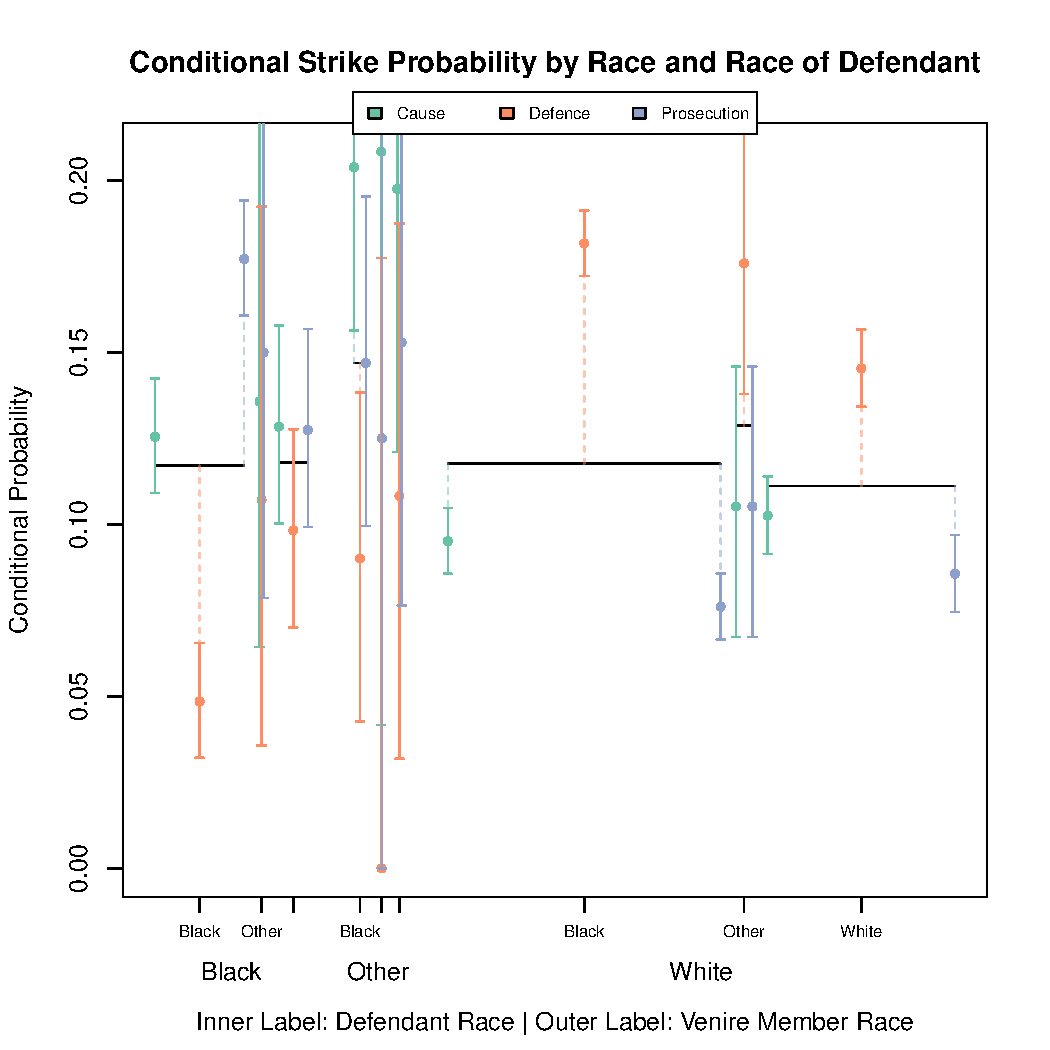
\includegraphics[width=0.7\textwidth]{RaceDefCI}
  \caption[Strikes by Racial Combination with Confidence
  Intervals (Sunsine)]{\footnotesize The plot of conditional strike probability by racial
    combination from Figure \ref{fig:racedefmob} with confidence intervals added. Note that many of the seemingly striking departures seen are
    insignificant when these confidence intervals are applied,
    especially for races other than black and white.}
  \label{fig:racedefci}
\end{figure}

While Figure \ref{fig:racedefmob} is quite suggestive, the widths of certain horizontal black lines, in particular those for venire members with a race other than white or black, suggest that some of the more extreme tendencies are simply a result of the greater variation of small samples. In order to see the true nature of the noted departures some incorporation of the expected variation is required. This is accomplished by the addition of approximate 95\% simultaneous multinomial confidence intervals using the \texttt{MultinomialCI} package in \R, which implements simultaneous confidence intervals for multinomial proportions following the method presented in (\cite{sison1995}). These confidence intervals can be seen in Figure \ref{fig:racedefci}.

As suspected, some of the results for the smaller sample sizes do not seem to be significant. However, the results for the larger groups, in particular for white venire members or black defendants, are significant. It should be noted that these simultaneous confidence intervals do not constitute a proper statistical test of the impact of race, but instead provide the viewer some sense of the expected variability in the data over repeated sampling. More rigorous testing requires controlling for the impact of confounding factors, as done by the modelling in Section \ref{sec:mods}.

Of course, it would be incorrect to conclude immediately that the cause of the racial patterns observed across these data sets is race itself. A plethora of attitudes associated with race could serve as legitimate cause for a peremptory challenge, as noted by Justice Byron R. White in the majority opinion in \textit{Swain v. Alabama} (\cite{swainvalabama}).

Without detailed transcripts detailing voire dire, it cannot be known if the aggregate pattern of removal is the result of racially based strikes, or whether the lawyers determined valid reasons for a peremptory challenge related to race. Striking a venire member due to their political affiliation, for example, would be allowed, and so racial heterogeneity could cause valid strikes to appear invalid. Such an ``ideological imbalance'' in racial political affiliations is actually present in this data set, and has been noted elsewhere in the literature (\cite{revesz2016}).

Consequently, answering the question of peremptory strike validity precisely requires that all available confounding factors be controlled. While such controlled modelling has already been completed for (\cite{StubbornLegacy}) and (\cite{PerempChalMurder}), no such modelling has been completed for the much richer and larger Jury Sunshine data set. The design of the mobile plot further motivates such multivariate regression by suggesting a particular form of model: the multinomial logistic regression model.

\subsubsection{Multinomial Logistic Regression}

The mobile plot used in Figure \ref{fig:racedefmob} displays the conditional distribution of a categorical variable with multiple levels given some combination of other variables. The natural model to complement this plot, then, would be a conditional multinomial model. Consequently, a multinomial log-linear regression model was fit to the data. The specific implementation of multinomial regression utilized was the \texttt{multinom} function in the \texttt{nnet} package in \R, which implements a method of fitting multinomial logistic regression models discussed in (\cite{nnet}).

For all models, the pivot outcome chosen was the probability of a venire member sitting on the final jury, in other words the probability their disposition was coded as \texttt{Kept}. Coefficients were then estimated using treatment contrasts against a black female venire member with Democrat voting tendencies in a case with a black female defendant. While the choice of race, gender, and political affiliation for the reference level was not deliberate, the choice of pivot outcome, that of a venire member being kept, was made in order to make the visualizations of model coefficients easily compared to previous visualizations. Choosing another pivot would have hidden its effect as the intercept, making comparison more complicated.

The mobile plots created in \ref{sec:visual} suggest two main features to investigate: the impact of venire member race in peremptory challenge use and the interaction between race and defendant race. Therefore a model of venire member race, political affiliation, gender, defendent gender, defendant race, and an interaction effect between venire member race and defendant race, called the full model, was fit. To test the interaction and race effects in the presence of all other variables, nested models excluding the interaction and excluding venire member race were also fit, called reduced models 1 and 2 respectively. The deviance residuals of all three models were used to perform ANOVA tests comparing the models. These can be see in Table \ref{tab:modcomp}, which compares the deviances of the different models sequentially when fit to the Sunshine data.

\begin{table}[h!]
  \centering
  \caption[Nested ANOVA Table Demonstrating the Importance of
  Race]{\footnotesize Comparison of models, displaying the residual deviance, residual degrees of freedom, differences, and p-values of these
    differences for adjacent models.}
  \label{tab:modcomp}
  \begin{tabular}{|c|c|c|c|c|} \hline
    \textit{Model} & \textit{Residual df} & \textit{Residual Deviance} & \textit{Difference} & $P(\chi^2)$ \\ \hline
    Reduced Model 2 & 55527 & 39496 &  &  \\
    Reduced Model 1 & 55521 & 39087 & 405 & ~0 \\
    Full Model & 55509 & 39023 & 67 & 1.4e-9 \\ \hline
  \end{tabular}
\end{table}

Even when controlling for defendant characteristics and the venire member's political affiliation and sex, the race of the venire member and its interaction with the defendant race are both highly significant at the $\alpha = 0.05$ level. This suggests that the rejection of venire members is, at least in part, based on their racial characteristics. Note that the residual deviance values indicate that this model is underdispersed, implying that the significant test results gained are conservative.

Due to its significance compared to the other models, the full model was taken as the final model to estimate the race effects with precision. Inspired by the dot-whisker plot (\cite{dotwhisker}), a custom dot-whisker plot was designed to display the model coefficients. This plot displays the coefficient estimates as points in the centre of a line, the endpoints of which give the associated confidence intervals. A vertical line is placed at zero to provide a reference for the sign and significance of different parameters. Modifying this concept to suit the multinomial regression data required grouping the different possible outcomes for each parameter spatially. The estimated coefficients for the different effects and their approximate 95\% confidence intervals, calculated using the standard errors of the coefficients and a normal assumption, are displayed using this modified dot-whisker plot in Figure \ref{fig:modallcoef}.

\begin{figure}[h!]
  \centering
  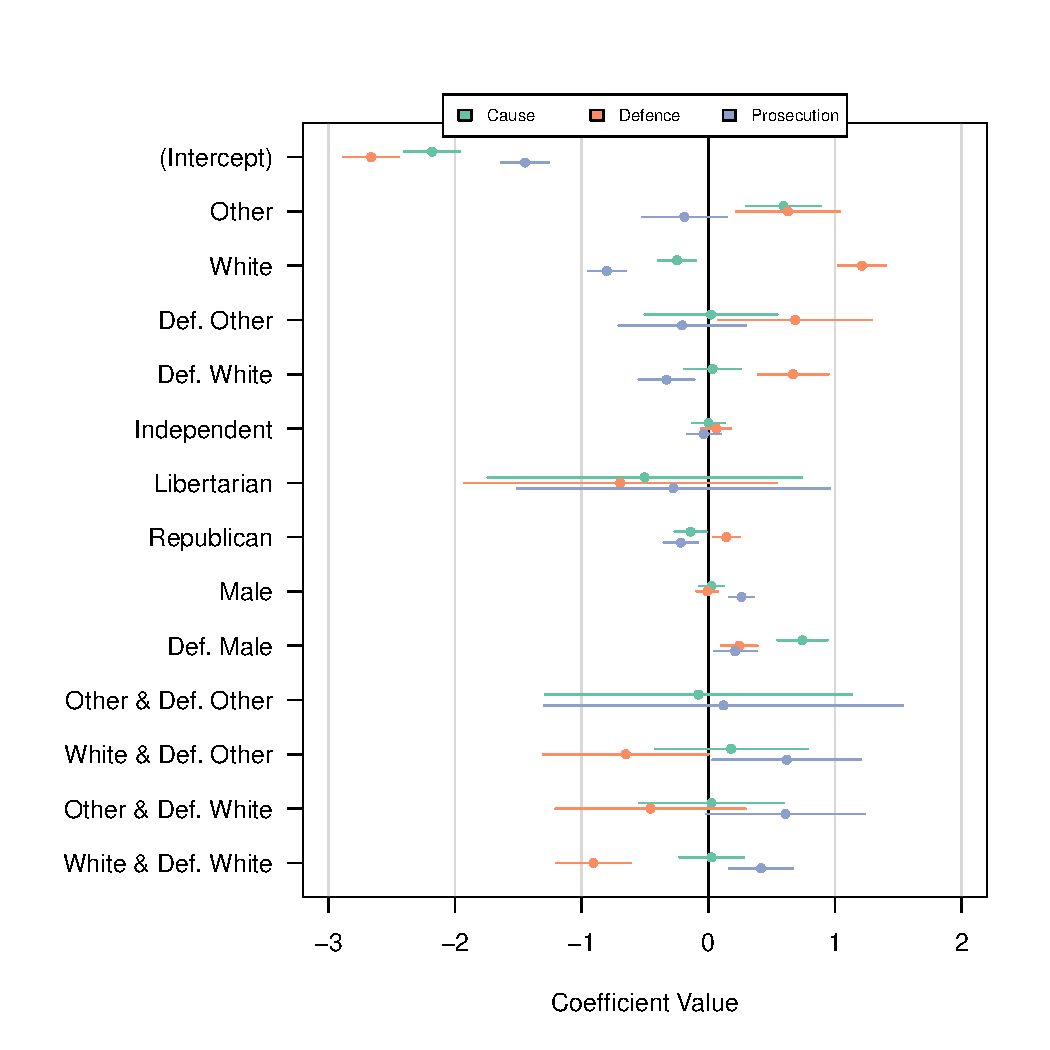
\includegraphics[scale=0.7]{AllModCoef}
  \caption[All Model Coefficients]{\footnotesize Model coefficients from the full model displayed using
    a dot-whisker plot. The lines indicate the confidence intervals while the central points indicate the point estimates of
    coefficients.}
  \label{fig:modallcoef}
\end{figure}

%\begin{figure}[h!]
%  \centering
%  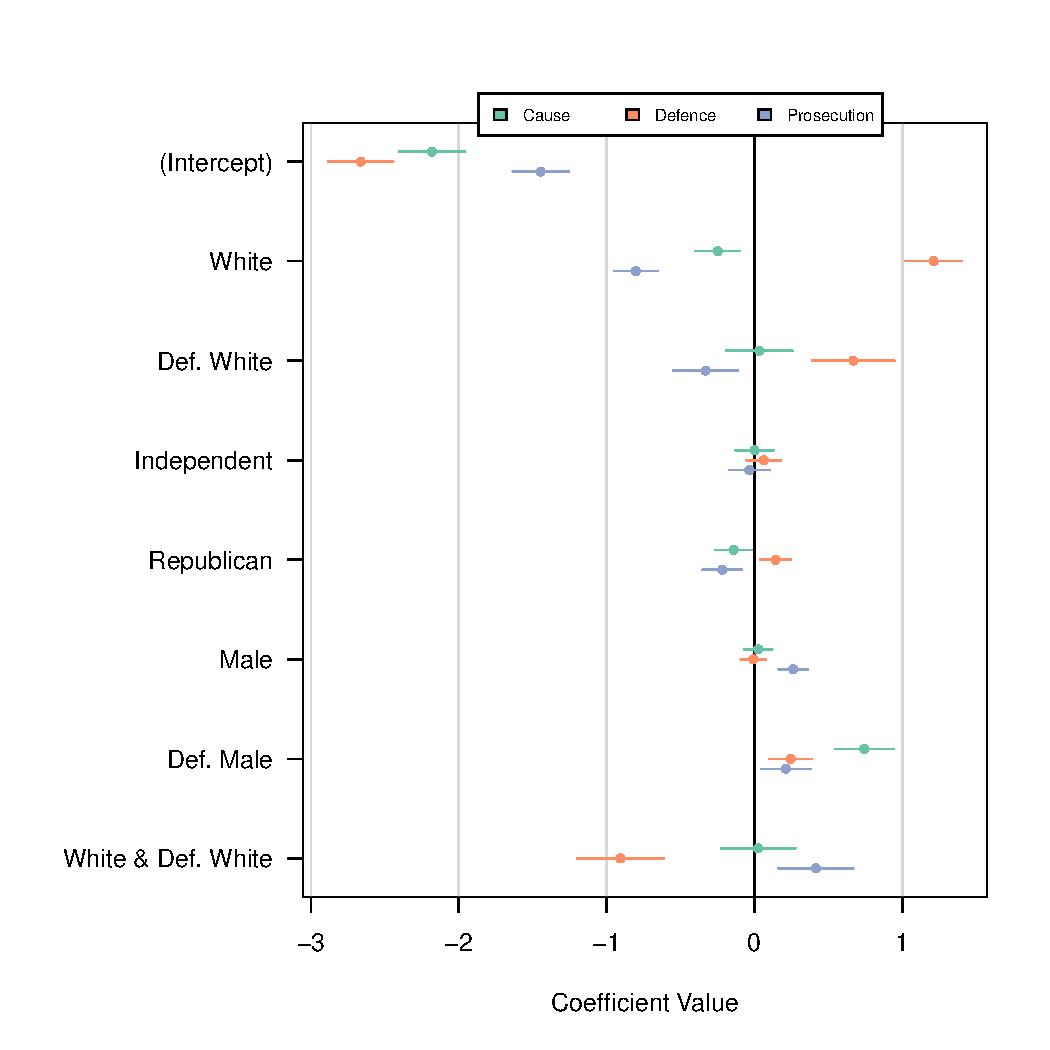
\includegraphics[scale=0.7]{SelectModCoef}
%  \caption[Select Model Coefficients]{\footnotesize Select model coefficients from the full model displayed using a dot-whisker
%    plot. The lines indicate the confidence intervals while the central points indicate the point estimates of coefficients.}
%  \label{fig:modselcoef}
%\end{figure}

The first noteworthy feature of this plot is the position of the coefficient estimates relative to the black line at zero. A coefficient to the right of the black line indicates that the factor corresponding to the coefficient increases the probability of the venire member disposition and a coefficient to the left indicates that the presence of said factor decreases the probability of the venire member disposition. The pattern of positive and negative values suggests the racial patterns noticed in the mobile plots were not the result of confounding with any recorded variables.

The variables which show the greatest significance and the characteristic oppositional tendencies of the prosecution and defence seen in Figure \ref{fig:racedefmob} are all race variables. White venire members, white defendants, and the interaction of white venire members and white defendants all have significant impacts on the probability of a venire member's removal by peremptory challenge. Furthermore, the prosecution and defence display opposite tendencies for these racial aspects and the magnitude of the defence coefficients is consistently greater than the prosecution for the race variables. This suggests that, on average, the defence is more sensitive to the racial aspects of the trial than the prosecution in the Sunshine data.

A quick survey of the prosecution peremptory challenge and challenge with cause coefficients shows far less agreement than seemed apparent in the mobile plots. Scanning from the top to the bottom, the cause coefficients match the prosecution for a few groups, but are generally different and often more similar to the defence than the prosecution. The suggestive pattern of matching prosecution strikes and causal strikes viewed in Figure \ref{fig:racedefmob} vanishes when controls are placed on possible confounders. In general, the cause strike coefficients are lower in magnitude than both the prosecution and defence, with the notable exception of the effect for male defendants, where it is significantly greater than both.

There are a number of more nuanced patterns present as well. Note that more venire members were kept than rejected in the Sunshine data, and so the negative intercept for all strikes is expected. More intriguing are the large differences between the different strike intercepts. These suggest that all three strikes are used differently in the pivot case, that of a female, black, Democrat venire member in a case with a female, black defendant. Crucially, the defence intercept is smaller than the prosecution, matching what was observed in Figure \ref{fig:racedefmob}, where the lowest defence strike probability occurred for black venire members in cases with black defendants. 

The coefficients for white venire members also match the expectations of Figure \ref{fig:racedefmob}. The defence attains its largest positive coefficient for white venire members and the prosecution its largest negative coefficient, suggesting white venire members in cases with black defendants are the most polarizing. These trends perfectly reflect the dominant effect of venire member race visible in Figure \ref{fig:racedefmob}. It seems that the defence is much more likely to reject a white venire member and the prosecution much less likely.

Slightly attenuating this pattern is the interaction effect between a white defendant and a white venire member. As noted in Figure \ref{fig:racedefmob}, there appears to be a tendency for the defence to prefer venire members of matching race to the defendant while the prosecution has a tendency to do the opposite. The white defendant coefficient, which is negative for the prosecution and positive for the defence, and the interaction effect for white venire members with white defendants, which is positive for the prosecution and negative for the defence, matches this observation exactly. Moreover, this seems to be significant based on the plotted confidence intervals. This suggests that, while the prosecution dominantly rejects black venire members and the defence dominantly rejects white venire members, the parties in the courts are sensitive to possible racial matches. The defence pattern is consistent with a strategy which aims to partially select venire members to match the defendant race, while the prosecution partially selects to mismatch.

Such racial patterns in the prosecution and the defence dominate all other effects. The political effect is minor, though consistent with the hypothesis put forward by (\cite{revesz2016}), with a preference for Republicans by the prosecution and Democrats by the defence.

\subsubsection{In the Stubborn and Philadelphia Data}

\begin{figure}[h!]
  \centering
  \begin{subfigure}{0.32\textwidth}
    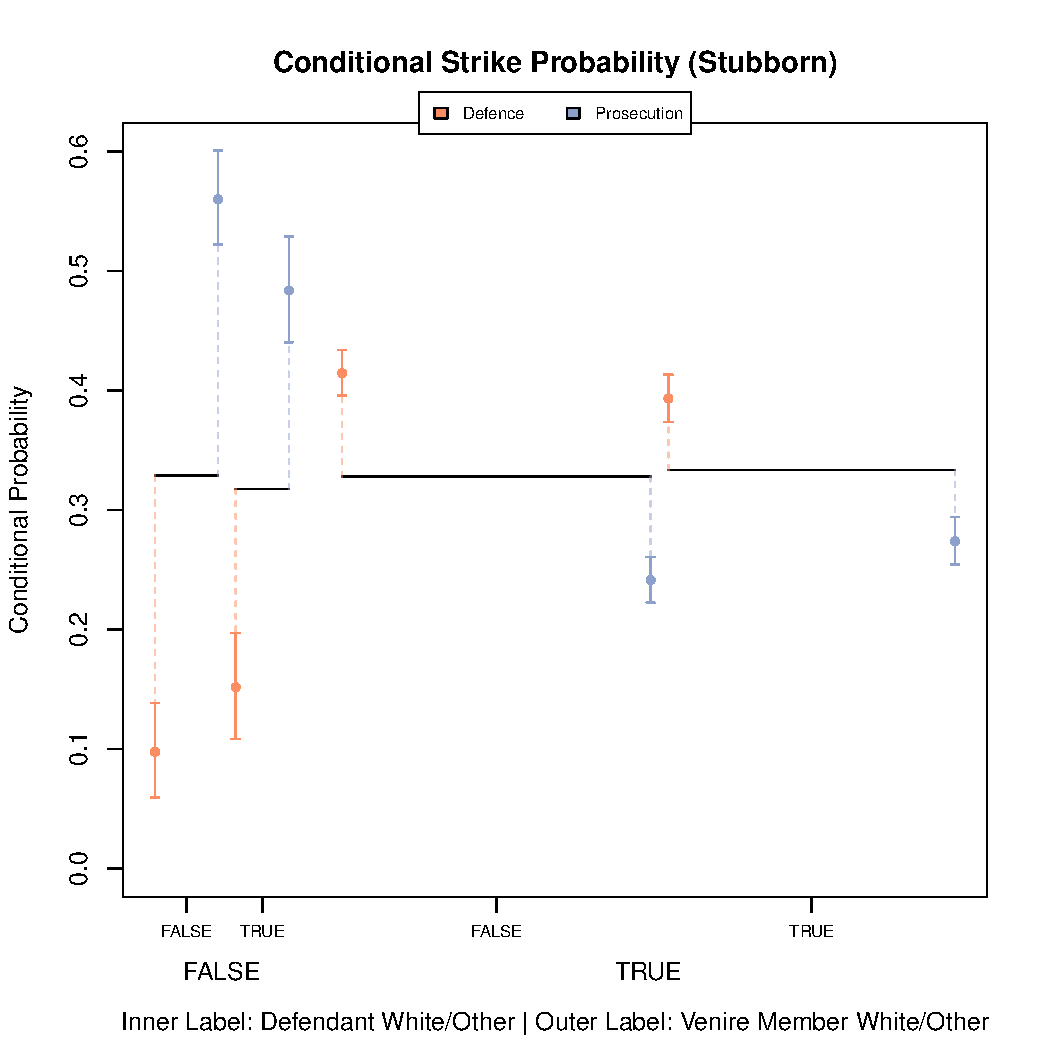
\includegraphics[scale = 0.32]{StubbornCompPlot}
    \caption{\footnotesize Stubborn strike pattern}
    \label{fig:stubcomp}
  \end{subfigure}
  ~
  \begin{subfigure}{0.32\textwidth}
    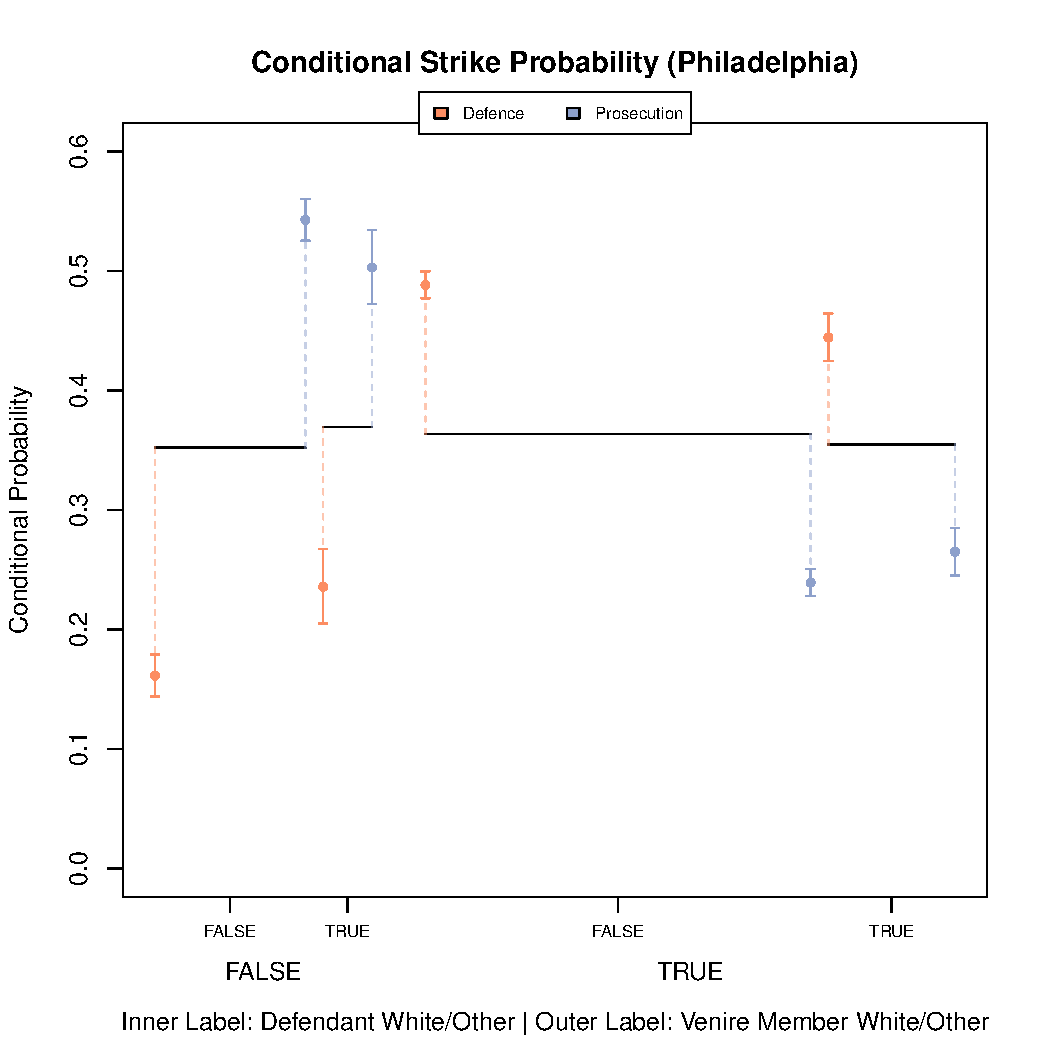
\includegraphics[scale = 0.32]{PhillyCompPlot}
    \caption{\footnotesize Philadelphia strike pattern}
    \label{fig:philcomp}
  \end{subfigure}
  ~
  \begin{subfigure}{0.32\textwidth}
    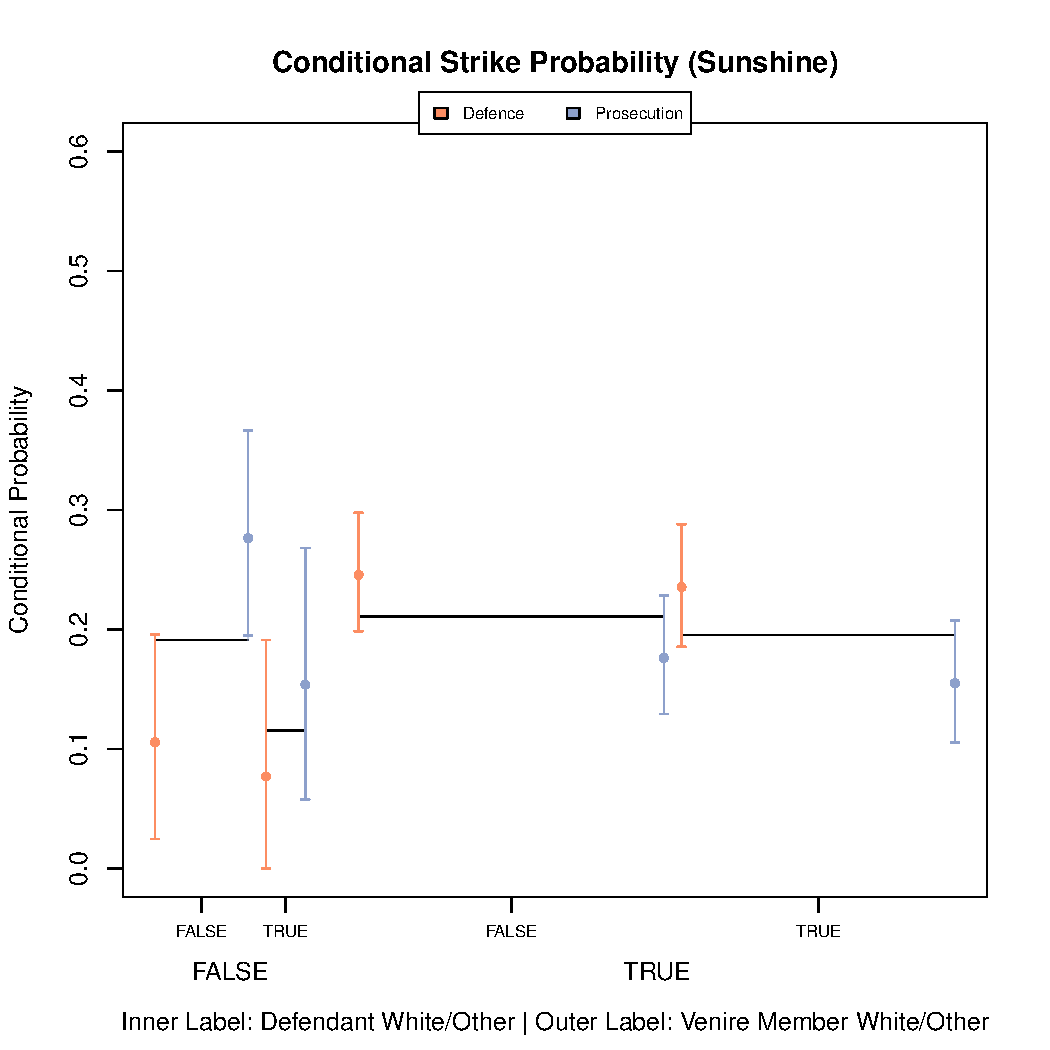
\includegraphics[scale=0.32]{SunshineCompPlot}
    \caption{\footnotesize Sunshine strike pattern}
    \label{fig:suncomp}
  \end{subfigure}
  \caption[Strikes by Racial Combination (All Capital Trial Data)]
  {\footnotesize The conditional probability of defence and prosecution peremptory challenge by race across all
    capital trials in all data sets. The pattern, though sometimes different in magnitude, is quite consistent across the three,
    despite the significant differences in the respective study sample universes.}
  \label{fig:racedefalldata}
\end{figure}

Already the utility of the mobile plot, and visualizations of the data in general, should be clear. A wealth of information is displayed very simply in Figure \ref{fig:racedefci}. However, the real power of this plot comes with the ability to quickly compare different data sets. Consider, for example, comparing all three data sets using Table \ref{tab:margrace}. In order to compare, the rows for each data set must be viewed and the numbers committed to memory before the reader moves to the appropriate row to compare values. While the simple four row and three column structure of this particular table make this rather straightforward, it becomes more difficult as the table grows in complexity. Compare this with a cursory glance at Figure \ref{fig:racedefalldata}, which makes the similarities of the data sets immediately clear despite the more detailed information represented. Note that the less detailed racial measurements in the Philadelphia data make these plots considerably different than Figure \ref{fig:racedefci}.

Despite the different study populations of these three data sets, all display similar patterns, with only the magnitudes of the strike rates differing. The mobile plot reveals several interesting aspects. The similar level of all black lines within each plot shows that in each data set, the aggregate probability of removal is similar across racial combinations, as was implied by Table \ref{tab:margrace}. However, these aggregate similarities hide the vastly and consistently different strategies of the defence and prosecution across all data sets. The defence has a tendency to retain black venire members, striking them at a lower rate than the other venire members, while the prosecution shows a pattern which mirrors that of the defence, removing more black venire members and fewer other venire members. In all data sets the gap between these probabilities and the expected strike rates are greatest for the black venire members in cases with black defendants.

It should be noted that the Sunshine data set looks most unique of the three, and this may be a result of the sampling method. While the Philadelphia data and Stubborn data both collected data which included multiple years and selected capital cases only, the Sunshine data was restricted to trials which occurred in 2011 and collected all cases. This small sample is the reason for the large confidence intervals present in Figure \ref{fig:suncomp}. This does not explain the overall lower strike rate observed in the capital trials in the Sunshine data, which is also visible in Table \ref{tab:margrace}. This departure may be of interest for future investigation.

\subsection{Trial Level Summary} \label{sec:casesum}

The control introduced by linear modelling ignores one critically important dependence that is present between jurors: the case. Cases share lawyers, judges, charges, and other important features which are not adequately controlled by the models fit in Section \ref{sec:mods}.  As it cannot be known why a particular venire member is struck, and modelling the patterns at the venire member level does not account for the close relationship between venire members on the same case, it is possible the aggregate patterns are the result of some effect other than persistent bias across trials. By aggregating the venire members by trial and viewing the racial strike behaviour at this level, insight into the impact of race on challenges at a more relevant scale is gleaned.

\subsubsection{Estimating Struck Juror Counts} \label{subsec:struckjur}

Aggregation required some synthesis, however. One gap present in the Sunshine data was the total count of defence and prosecution strikes for each trial. This variable is of minor importance for modelling the individual venire members, but it is of major interest when viewing the trials themselves. While counts of these strikes were provided in the data, there were many missing values, or values inconsistent with the number of associated venire members in the data. For example, many of the recorded values in these columns were zero even when venire members associated with that trial were marked as struck.

To remedy this,  counts of struck venire members with particular characteristics, for example race, were computed for each trial. To provide an estimate of the total number of venire members struck by each party, these counts were summed for one particular variable, typically gender. This sum was then compared to the recorded value for that party's removed count. The greater of the two values was kept as an estimated count to be used in analysis. For both the prosecution and the defence, about 80\% of the sum and recorded values matched exactly and about 18\% of the recorded values were less than the sum. This suggests some incompleteness for the remaining 2\% of the data.

\subsubsection{Visualizing the Racial Trends} \label{subsec:vistrend}

Motivated by the plots in the \texttt{extracat} package in \R (\cite{extracat}), in particular the \texttt{rmb} plot, the ``positional boxplot'' was developed to display the strike tendencies across trials. The data visualized by the positional boxplot consists of three parts: a categorical variable and two integer counts which have many duplicates in the data. At each unique combination of these counts observed, a box is placed with two features: an area proportional to the total number of observations with the corresponding counts, and subdivisions with horizontal lengths proportional to frequencies of each level of the categorical variable that occurs with that specific integer combination. In this case, the categorical variable is the defendant race and the counts are the peremptory challenges used by the defence and prosecution, displayed in Figure \ref{fig:trialprodef}.

\begin{figure}[h!]
  \centering
  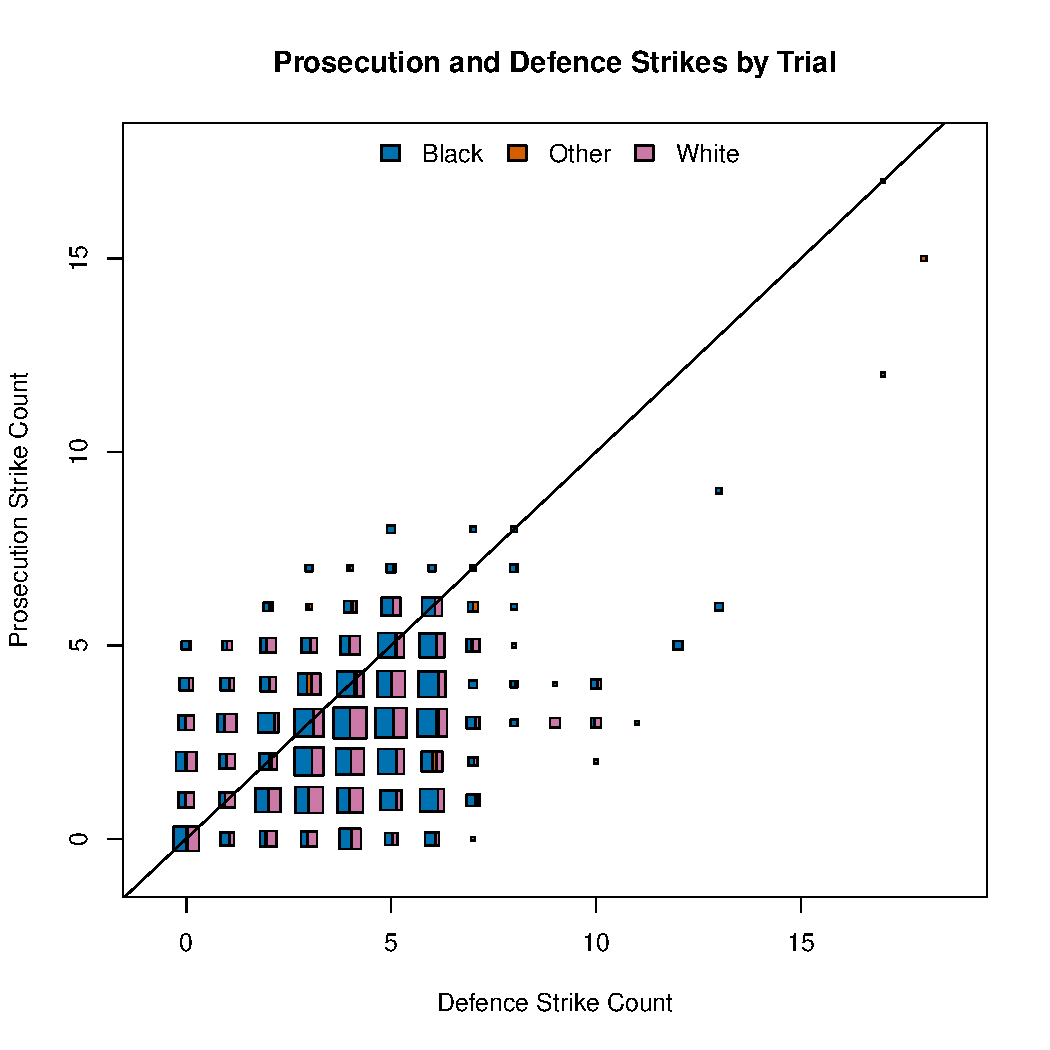
\includegraphics[scale=0.7]{DefProStrikesTrial}
  \caption[Prosecution and Defence Strikes by Trial]{\footnotesize The positional boxplot of strikes by race of defendant for the
    Sunshine data. There does not seem to be a dependence of strike counts on the defendant race, the boxes look similar across
    the entire plot.}
  \label{fig:trialprodef}
\end{figure}

While the internal box patterns look rather similar everywhere, split somewhat evenly between black and white defendants, their areas are quite revealing. The greater area of boxes below the diagonal line demonstrates clearly the tendency for the defence to use more peremptory challenges than the prosecution in a given case.

However, this plot fails to account for the total number of black and white venire members presented to the court in each of the trials. We would expect these numbers to be very different in the Sunshine data; the different lengths of the horizontal black lines in Figure \ref{fig:racedefmob} indicate that a sizeable majority of the venire members are white. To account for this, the raw strike counts were normalized into proportions of venire members of the corresponding race. The resulting scatterplots of these proportions by trial are displayed in Figure \ref{fig:defproprop}.

\begin{figure}[h!]
  \centering
  \begin{subfigure}{0.45\textwidth}
    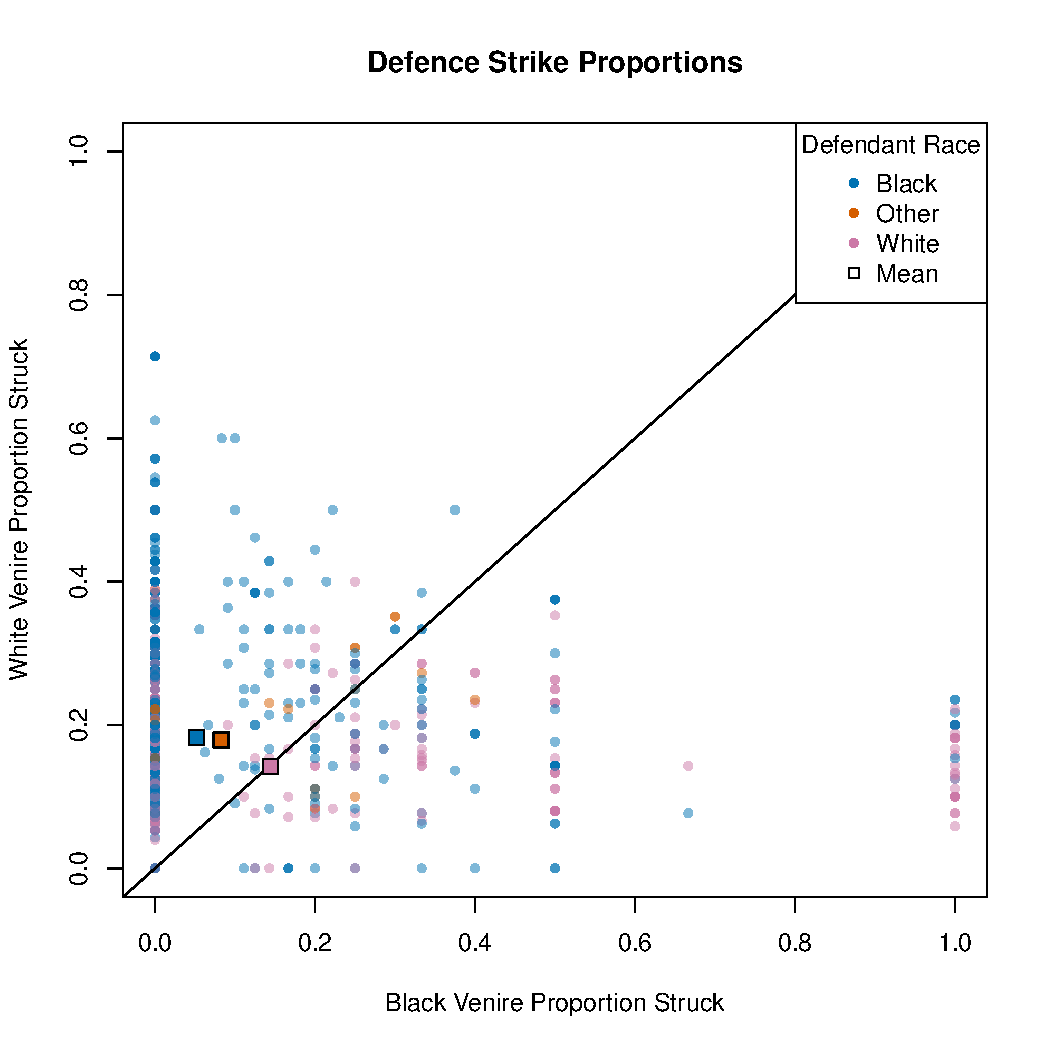
\includegraphics[scale = 0.45]{DefStrProp}
    \caption{\footnotesize Defence proportion venire removed}
    \label{fig:defraceprop}
  \end{subfigure}
  ~
  \begin{subfigure}{0.45\textwidth}
    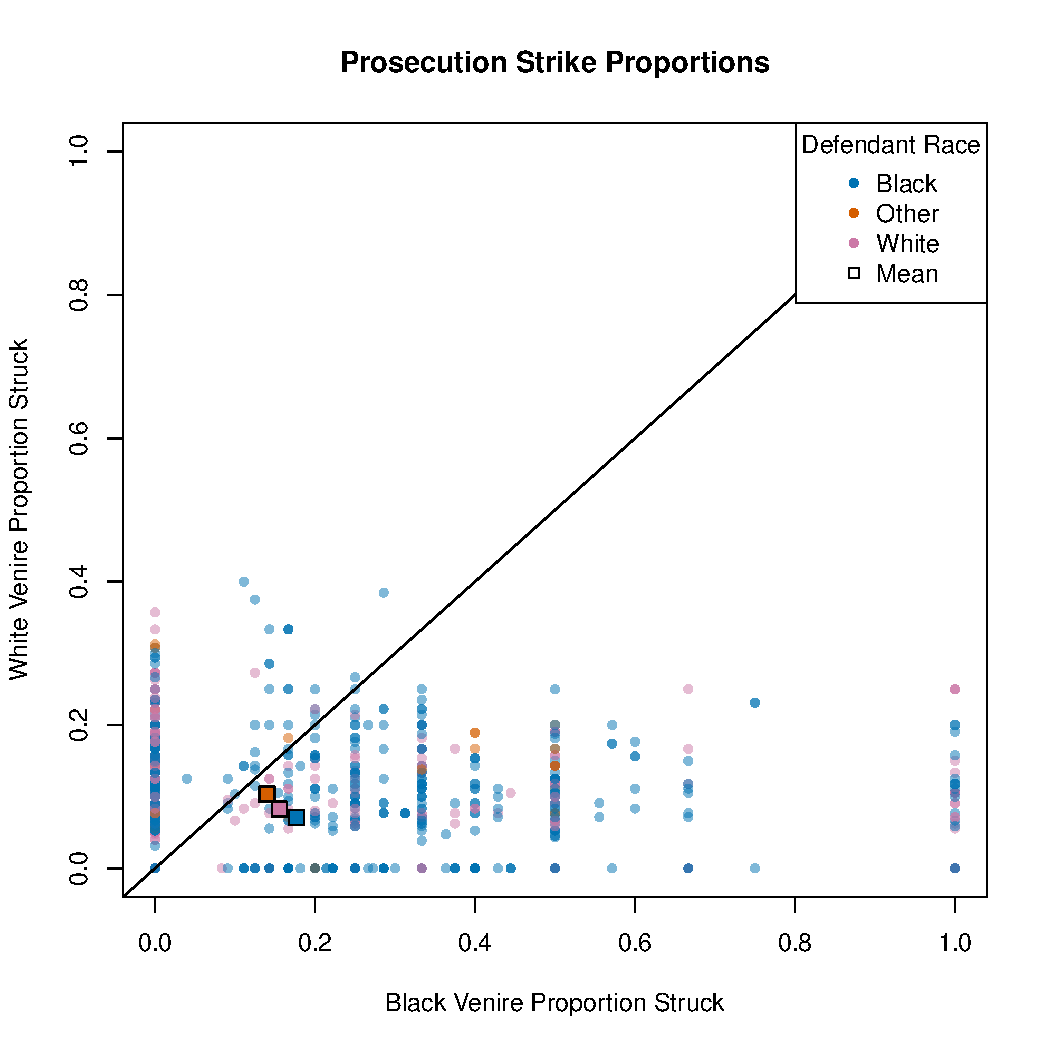
\includegraphics[scale = 0.45]{ProStrProp}
    \caption{\footnotesize Prosecution proportion venire removed}
    \label{fig:proraceprop}
  \end{subfigure}
  \caption[Racial Strike Proportions by Party]
  {\footnotesize Scatterplots of venire proportion removed by race for both the defence and prosecution.}
  \label{fig:defproprop}
\end{figure}

Here, the prosecution and defence biases are clear. The prosecution never strikes more than 40\% of white venire members presented, and on average strikes a greater proportion of the black venire than the white venire. The defence, in contrast, regularly strikes more than 40\% of the white venire, and on average strikes a greater proportion of the white venire members than the black venire members. This reinforces the observations made in Section \ref{sec:mods}, indicating that these mechanics operate at the trial level, not just the venire member level. More crucially, the high variation visible in Figure \ref{fig:defproprop} suggests that the aggregate patterns described here and in Section \ref{sec:mods} may be inadequate to describe any individual case.

This plot also reveals a fundamental difference in inclusion of minority and majority groups in juries. The aggregate statistics indicate that the black venire members are a minority, and Figure \ref{fig:defproprop} suggests that as a consequence, it is common that a majority or all of the potential black jurors will be struck by peremptory challenge. There is not a single case where all of the majority white venire members are struck, suggesting the exclusion of white venire members is rare, if not impossible. Whether these peremptories are being used legitimately, the ultimate consequence of their use is the exclusion of minorities from the juries of cases with minority defendants. Given the tarnished history of peremptory challenge for deliberate exclusion, this pattern is concerning.


The visual tools and models presented here support the dominant analysis in the literature. There is a persistent racial bias in the exercise of peremptory challenges in the Sunshine data set, and an analogous pattern appears to be present in the Philadelphia and Stubborn data sets. The prosecution tends to remove more racial minority venire members than expected and fewer white venire members than expected. The defence tends to have the opposite strategy. This pattern is not only seen in aggregate in Section \ref{sec:visual}, but is visible in the trial summaries presented in Section \ref{sec:casesum}. The impact of race remains apparent even when other legitimate factors such as political affiliation are controlled.

Beyond detecting these patterns, this work demonstrates the strengths of visual analysis. The first of these is the utility of carefully constructed visualizations to compare the strike patterns across multiple data sets. The similarities between the Stubborn, Philadelphia, and Sunshine data sets are immediately clear when visualized appropriately. This is critical in the examination of peremptory challenges, as it allows for a comparison of their use across studies with radically different study populations so long as analogous data is collected. In this case, the strength of the similarities observed between these data sets when visualized with the mobile plot suggests the pattern of racial preferences is not a local phenomenon in location or time, but is a reflection of a strategy utilized by the prosecution and defence in jury trials generally.

Another strength of the mobile plot is to motivate modelling. The multinomial regression models from Section \ref{sec:mods} were created to fit models analogous to the mobile plots generated to explore the data. That the findings of the models matched the analysis of the mobile plots almost exactly demonstrates the analytical utility of these plots. The models motivated by Figure \ref{fig:racedefmob} allowed for the estimation of effects in the Sunshine data controlling for possible legitimate confounders, giving coefficient estimates consistent with those generated previously for other data sets, such as the Stubborn and Philadelphia data.

Visualising these coefficients with the dot-whisker plot made a number of more nuanced patterns obvious. The first of these is the greater sensitivity of the defence to the racial aspects of a trial than the prosecution; the race of the venire member has a greater impact on the defence's probability of rejection than the prosecution's. The second pattern is the tendency of race matching by the defence and race contrasting by the prosecution. This aggregate pattern also seems to be reflected in the trial level summary of the data, which suggests that this trend is a reflection of decision making across trials.

Of course, as suggestive as these patterns are, and as spotted as the history of peremptory challenges is with controversy, none of this can say definitively whether the individuals rejected from the Sunshine venires were rejected inappropriately due to their race. Without detailed descriptions of the bias of the population as a whole, such judgements on the propriety of strikes simply cannot be made, and whether these racial strike patterns are simply the result of legitimate strikes for reasons related strongly to race cannot be ascertained. Additionally, the highly variable nature of peremptory challenge use indicates that these aggregate trends are highly inadequate to predict the behaviour of lawyers in any particular case.

Despite this limitation, the final scatterplots suggest a criticism of peremptory challenges independent of these concerns and consistent with the source of controversy for \textit{Batson v. Kentucky}, \textit{Swain v. Alabama}, and \textit{R. v. Stanley}. Peremptory challenges frequently remove all representatives of minority groups from the venire. This prevents minority participation in a panel meant to represent the conscience of their community, corroding a critical function of the jury and creating a group sceptical of the operation of the legal system. While the smaller sizes of minority groups and their relationship to the majority may lead to their under-representation for reasons other than peremptory challenges, a graphical exploration shows definitively that a component of their under-representation is peremptory challenges. Minority groups are fully struck from the venire by peremptories far more often than majority groups.

All of this paints a bleak picture of the use of peremptory challenges in the modern jury selection process. Without additional work, it is impossible to say with certainty whether the racial patterns observed here and elsewhere are due to racial prejudice by the court, but one may ask the question of whether that matters. As Lord Chief Justice Hewart said in \textit{R. v. Sussex Justices}

\begin{quote}
  Justice should not only be done, but should manifestly and undoubtedly be seen to be done
\end{quote}

The visualisations of this paper have made much seen, but it is doubtful that what has been seen looks like justice.


%%%%%%%%%%%%%%%%%%%%%%%%%%%%%%%%%%%%%%%%%%%%%%%%%

\bibliographystyle{apalike}
\bibliography{myReferences}

\end{document}